\documentclass[11pt]{article}

% Language setting
% Replace `english' with e.g. `spanish' to change the document language
\usepackage[english]{babel}
\usepackage[table,xcdraw]{xcolor}

% Set page size and margins
% Replace `letterpaper' with`a4paper' for UK/EU standard size
\usepackage[a4paper,top=2cm,bottom=2cm,left=3cm,right=3cm,marginparwidth=1.75cm]{geometry}

% Useful packages
\usepackage{amsmath}
\usepackage{graphicx}
\usepackage[colorlinks=true, allcolors=blue]{hyperref}
\usepackage[most]{tcolorbox}
\usepackage[normalem]{ulem}
\useunder{\uline}{\ul}{}
\usepackage{lscape}
\usepackage{longtable}
\usepackage{spverbatim}
\usepackage{listings}
\lstset{breaklines=true} 
\usepackage{upquote}
\usepackage{biblatex}
\usepackage{subcaption}
\usepackage{graphicx}
\usepackage{diagbox}
\usepackage{mathabx}
\usepackage{float}
% \addbibresource{trama.bib}
\bibliography{trama.bib}
\title{Trope detection using LLaMA 2 \\

% \begin{tcolorbox}[colback=green!5!white,colframe=green!75!black,title=Example]
%   Predicting the Price of Food from Restaurant Menus
% \end{tcolorbox}

}
\author{Shantam Raj}

\begin{document}
\maketitle

\begin{abstract}
LLaMA 2 \cite{touvron_2023_llama} demonstrates promising capabilities in the detection of tropes\footnote[1]{A narrative trope is a common or overused element in storytelling that helps to convey certain themes or ideas. These can include things like the "chosen one" trope, where a protagonist is destined for greatness, or the "fish out of water" trope, where a character is placed in an unfamiliar environment. Narrative tropes can be used to create a sense of familiarity or comfort for audiences, but they can also be subverted or played with in order to add complexity and depth to a story.} within narrative text. Given the extensive array of tropes cataloged by the TVTropes\footnote[2]{https://tvtropes.org/} community and the inference time and computational resources needed to run LLaMA 2 it becomes crucial to employ complementary techniques for trope filtration within narratives. Subsequently, we can query the language model to ascertain the validity of identified tropes. This strategy not only optimizes resource utilization but also elevates the precision of trope identification in the context of storytelling.
\\
This preliminary research offers a novel perspective on the automated extraction of tropes from narratives. The findings from this early stage study provides insights for researchers, authors, and enthusiasts seeking to gain a deeper understanding of storytelling conventions and their applications in the digital age through the lens of tropes and leveraging Large Language Models (LLMs).
\end{abstract}

\section{Introduction}
I want to find out if it is possible to use semantic similarity and prompting to extract tropes from shortstories. It broadly utilizes information retrieval, embeddings, prompting and LLMs. The input is a short story/flash fiction and the output is a list of tropes.

\section{Data set}

\subsection{Stories}

\subsubsection{Shortstory files}
This dataset was curated manually from the following sources - 
\begin{itemize}
  \item Project Gutenberg - https://www.gutenberg.org/
  \item Classic Short Stories - https://www.classicshorts.com/
  \item Literature Collection - http://www.literaturecollection.com/
  \item The New Yorker Flash Fiction - https://www.newyorker.com/books/flash-fiction
\end{itemize}
The dataset was curated manually because of lack of clean dataset of human authored shortstories or flash fiction. The context of LLaMA 2 was a deciding factor for the length of stories. It has a maximum context of 4096 tokens and using `rope scaling' in the transformer version of LLaMA 2, the context can be doubled to 8192 tokens. Majority of the stories fit in that context window.

Every shortstory is a separate file in the ``dataset" folder in the repository\footnote[3]{\url{https://github.com/armsp/trama}}. The structure of the text in each story file is described in Appendix \ref{appendix:a}.

\subsubsection{Story Summaries}
Summaries of stories were generated using `GPT 3.5 Turbo 16k" at two different temperatures - 0.7 and 1. See \href{https://github.com/armsp/trama/blob/main/story_dataset_maker.ipynb}{story\_dataset\_maker.ipynb} and \href{https://github.com/armsp/trama/blob/main/story_summaries.ipynb}{story\_summaries.ipynb} for the steps used to create the dataset and summaries. There are many ways to summarize a story. See Appendix \ref{appendix:f}. Tropes are essentially an outcome of plot and character developments hence the prompt used was the following - 
\begin{lstlisting}
  [{"role": "system", "content": "You provide a detailed summary of the given story. Focus on the plot line and character development."},
  {"role": "user", "content": <story>}]
\end{lstlisting}
Figure \ref{fig:tokens} shows the token distribution of story and summary text. See \href{https://github.com/armsp/trama/blob/main/visuals.ipynb}{visuals.ipynb} on how the tokens were calculated.
\begin{figure}[h]
\caption{Token histograms}
\label{fig:tokens}
  \begin{subfigure}[t]{.45\textwidth}
  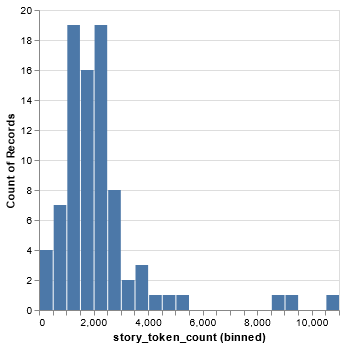
\includegraphics[scale=0.5]{story_tokens.png}
  \caption{Token histogram of shortstories (bin size = 500 tokens)}
% \end{figure}
  \end{subfigure}%
  \hfill     
% \begin{figure}[h]
  \begin{subfigure}[t]{.45\textwidth}
  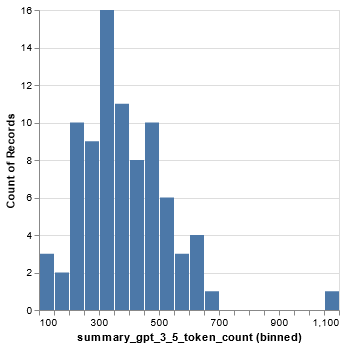
\includegraphics[scale=0.5]{summary_tokens.png}
  \caption{Token histogram of shortstory summaries generated at temperature of 0.7 by `gpt 3.5 turbo 16k' (bin size = 50 tokens)}
  \end{subfigure}
% \end{figure}
  \begin{subfigure}[t]{.95\textwidth}
  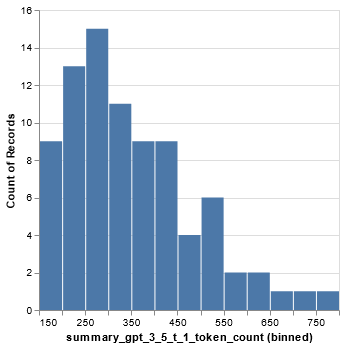
\includegraphics[scale=0.5]{summary2_tokens.png}
  \caption{Token histogram of shortstory summaries generated at temperature of 1 by `gpt 3.5 turbo 16k'(bin size = 50 tokens)}
\end{subfigure}
\end{figure}

\subsection{Tropes}
\subsubsection{Trope Definitions}
The tropes dataset is a subset of the original tvtropes dataset \cite{gala-etal-2020-analyzing}. See Appendix \ref{appendix:b} for an example of the first few rows of the dataset.

\href{https://github.com/armsp/trama/blob/main/dataset/my_tropes.csv}{my\_tropes.csv} file consists of examples of the selected tropes from literature and goodreads. In total we select 500 tropes to study. 400 of the tropes are the most common tropes in literature and goodreads (the selected tropes are common to both). Similarly, the remaining 100 tropes are the less common tropes from literature and goodreads. See Appendix \ref{appendix:c} for an example of the first few rows of the dataset. See \href{https://github.com/armsp/trama/blob/main/select%20tropes.ipynb}{select\_tropes.ipynb} for the steps used to prepare the dataset.

\subsubsection{Trope Examples}
The 500 tropes selected above were used to extract examples of those tropes from literature and film examples\footnote[1]{the tvtropes dataset has examples of tropes that contain the trope names, titles, and examples across each form of media - tv, film and literature}. In total there are 1,86,899  examples. Literature and film examples were chosen and Tv was ignored. See \href{https://github.com/armsp/trama/blob/main/trope_examples_dataset.ipynb}{trope\_examples\_dataset.ipynb} for the steps used to create the dataset.
\\
\\
\noindent The Tvtropes dataset was chosen because it is the only known textual dataset of tropes.
% \begin{tcolorbox}[colback=green!5!white,colframe=green!75!black,title=Example]
%   I chose the \textit{Uber Eats Menus} data set.
%   The dataset was constructed by scraping the menu text and prices of food advertised by restaurants on Uber Eats.
%   Each menu item also comes with a restaurant ID and user reviews.
%   I think this is the best dataset for this task because it is the biggest and most diverse dataset.
%   I could have used the \textit{Open Recipes Data Dump} instead, which would have made the task about prediction from the recipe text instead of the menu description.
% \end{tcolorbox}

\section{Preprocessing}
It was not necessary to perform substantial pre-processing because of the nature of the models used. The tokenization is generally part of open source pipelines. The only pre-processing that I perform is to remove leading and trailing whitespace,  `\textbackslash t', `\textbackslash n', and `\textbackslash r' from the tropes and stories dataset. 

\section{Experiments}
My first attempt was to use prompt engineering to extract all the tropes. However prompting is not an exact science. Since this was a specialized task, to come up with the best possible prompt I explored many combinations of System Prompts and User Messages to find the best combination. However I realized after spending a lot of time on manually finding the best pair, that this is not the best use of time. Prompting will never output all the tropes in a given story since its a very broad task. LLMs are most useful when the prompts are very specific. However in that time I was able to make the following matrix of System Prompt and User Message combinations. See Appendix \ref{appendix:e} for System Prompts and User Messages.

\begin{table}[H]
  \resizebox{3cm}{!}{%
  \begin{tabular}{ll}
  \multicolumn{2}{l}{\textbf{Legend}}           \\
  \cellcolor[HTML]{32CB00} & Correct and usable \\
  \cellcolor[HTML]{FFFF00} & Limited usability  \\
  \cellcolor[HTML]{FF0000} & Wrong and unusable
  \end{tabular}%
  }
\end{table}
\vspace{-2em}
\begin{table}[H]
  
  \resizebox{\textwidth}{!}{%
  \begin{tabular}{|l|l|l|l|l|l|l|l|l|l|l|}
    % \diagbox[]{User msg}{System Prompt}&
  \textbf{\tiny User Msg/System Prompt} &
    \textbf{S1} &
    \textbf{S2} &
    \textbf{S3} &
    \textbf{S4} &
    \textbf{S5} &
    \textbf{S6} &
    \textbf{S7} &
    \textbf{S8} &
    \textbf{S9} &
    \textbf{S10} \\ \hline
  \textbf{U1} & 
    \cellcolor[HTML]{FFFF00} &
    \cellcolor[HTML]{FFFF00} &
    \cellcolor[HTML]{FE0000} &
    \cellcolor[HTML]{FE0000} &
    \cellcolor[HTML]{FE0000} &
    \cellcolor[HTML]{FE0000} &
    \cellcolor[HTML]{32CB00} &
    \cellcolor[HTML]{FFFF00} &
    \cellcolor[HTML]{FFFF00} &
    \cellcolor[HTML]{FFFF00} \\ \hline
  \textbf{U2} &
    \cellcolor[HTML]{FE0000} &
    \cellcolor[HTML]{F8FF00} &
    \cellcolor[HTML]{FFFF00} &
    \cellcolor[HTML]{FFFF00} &
    \cellcolor[HTML]{32CB00} &
    \cellcolor[HTML]{FFFF00} &
    \cellcolor[HTML]{FFFF00} &
    \cellcolor[HTML]{32CB00} &
    \cellcolor[HTML]{FFFF00} &
    \cellcolor[HTML]{FE0000} \\ \hline
  \textbf{U3} &
    \cellcolor[HTML]{FFFF00} &
    \cellcolor[HTML]{FFFF00} &
    \cellcolor[HTML]{FE0000} &
    \cellcolor[HTML]{32CB00} &
    \cellcolor[HTML]{FFFF00} &
    \cellcolor[HTML]{FE0000} &
    \cellcolor[HTML]{FFFF00} &
    \cellcolor[HTML]{FE0000} &
    \cellcolor[HTML]{FFFF00} &
    \cellcolor[HTML]{FFFF00}
  \end{tabular}%
  }
\end{table}
My second experiment was to use semantic similarity to identify tropes in stories. The idea was to compute cosine similarity of summaries of stories with examples of tropes. For that, I used USE\cite{cer_2018_universal} to get embeddings for summaries, full text of stories and examples of tropes. 
I chose USE because in my experience for longer texts and paragraphs it had performed better than other models like Sentence Transformer. After getting the cosine similarity of each story with the trope examples, I filtered and then selected the top ten tropes for each story. Finally I asked LLaMA 2 itself if those tropes are indeed present in the story.
\\
Using semantic similarity on the full story text worked better than on summaries of the story. However it is important to point out that the thresholds are not the same for filtering the tropes. 
After filtering the tropes using similarity threshold I selected the top ten tropes for each story. See \href{https://github.com/armsp/trama/blob/main/dataset/story_with_tropes_by_similarity.csv}{story\_with\_tropes\_by\_similarity.csv} for the result. 
\\
After that I used LLaMA 2 13b to ask if those tropes actually exist in the stroy text. LLaMA 2 13b is not adept at outputting JSON. I tried numerous prompts and temperatures to get it to output JSON that can be easily parsed, but it always failed. I could not run my fork of `guidance' \ref{fork} to get stable output due to time constraints. This problem also led me to another project - \href{https://github.com/ggerganov/llama.cpp/tree/master/grammars}{llama.cpp grammar} that could be useful for the task. Eventually I wrote my own simple parser to parse the LLM output as a dictionary that could be saved as a column in the final dataset file. However by then the prompt had changed too the output style of LLaMA 2 changed dramatically and never went back to the original output.\\
I could not run the same analysis on the 70b model which I expect to be more accurate and to better follow the instructions. However, after waiting for 3 days after submitting the job on Euler to get enough GPUs to run the model, I had to give up on the idea. 

\section{Evaluation}
This is understandably the most important but also the most difficult task. Initially the plan was to perform a manual validation of tropes identified through semantic similarity. However, that proved to be infeasible. Therefore I used LLaMA 2 itself to ask if a trope exists in the story. LLaMA 2 13b gets somethings correct and some wrong.

There are also some very good examples where it identifies tropes that you wouldn't think of in the first place.\\
\textbf{Correct identifications}\\
(Story Title - Trope with reason for trope in the story - Comments)

\textit{Where are you? - The story's use of the "Verbal Irony" trope, where the words and actions of the characters have a different meaning than their literal meaning, such as the husband's "Hello? Hello?" calls, which are not actually a request for the wife's location, but a way for him to assert his power and control over her.} - This is a correct identification.
\\
There are certainly many tropes that LLaMA 2 13b gets wrong. The following are just some of the examples:
\\
\textbf{Wrong identifications}\\
(Story Title - Trope : Reason for trope in the story - Comments)
\begin{itemize}
  \item \textit{A Retrieved Reformation - The Faked Death: Jimmy "dies" as Ralph D. Spencer and is reborn as Jimmy Valentine to escape his criminal past and start a new life.} - This is clearly a wrong assessment of the story.
  \item \textit{The Boss - The Masked Face: The woman's face is masked in shadow, adding to the story's mystery and potential for hidden motives.} - Sometimes it thinks purely aesthetic choices as tropes.
  % \item \textit{Where are you? - The "Unseen Observer" trope, as the wife is often described as being "elsewhere" in the house, even though she is physically present in the same space as the husband.} - This is also not a correct assessment.
\end{itemize}
% Finally, for the most accurate results I used the largest LLaMA 2 model to ask if a given trope exists in a story.\\
% \\
I observed a strange phenomena, where LLaMA 2 13b would correctly list some tropes present in a story - when the tropes were not listed themselves to be checked. However, when asked specifically if a certain trope (tropes filtered using semantic similarity) existed then it always replied in affirmative and found reasons (even if incorrect) to justify it's reasoning. 
See the notebook \href{https://github.com/armsp/trama/blob/main/trope_validator_13b.ipynb}{trope\_validator\_13b.ipynb} for more examples and until the parser runs before the language model reaches the limit of its output and stops outputting midway which leads to parser failure.

% In general, the model determined that most of the tropes didn't actually exist. This is a plausible result and has been discussed in Section \ref{discussion}. 
\section{Outcome}
\begin{itemize}
  \item In terms of idea, I wanted to show that stories are a nuanced representation of multiple tropes in general. This was an original idea and worked very well for semantic similarity at the story level. However, the results were not so good for summaries.
  \item This is a valuable first step towards literary analysis of narratives -
  \begin{itemize}
    \item we can explore augmenting AI writing platforms for authors using insights from this project
    \item we can study evolution of tropes in works of narratives over time
  \end{itemize}
  \item A dataset of tropes (selected) for shortstories (lack of GPUs prevented running the 70b model for validation). 
  \item This analysis and pipeline can be made more robust and run on a larger set of stories while using the full tropes dataset to make a more complete dataset of tropes in stories.
  \item This is the only work as of now that explores using LLM for this task and also shows that LLMs are indeed useful for the task. 
  \item All the experiments and code is open sourced on GitHub.
  \item My fork of `guidance'\footnote[2]{https://github.com/armsp/guidance/blob/main/guidance/llms/transformers/\_llama.py}\label{fork} works with chat versions of LLaMA 2 and can output JSON that can be parsed. However a thorough testing needs to be done and it fails on JSON that has arrays. Please see Section \ref{formattedoutput} for the reason.

\end{itemize}

\section{Future work}
\begin{itemize}
  \item The task of querying the LLM for the existence of a certain trope can be made faster by optimizing the semantic similarity pipeline. Currently it utilizes batch input and vectorized calculations. However the end to end analysis pipeline is still quite slow.
  \item Different tropes also do not have similar number of examples. Therefore coming up with a more robust ranking approach will help in correctly identifying tropes.
  \item The most important task that we can also work on is how to represent stories themselves for the semantic similarity task. Representing the whole story as a vector embedding is perhaps not the best approach. Their length also dictates how diluted the embeddings are. To mitigate that I came up with the approach to summarize the story focusing on plot and character developments because tropes are centered around plots and characters. However this can be ``finetuned'' more such that extracting tropes becomes more accurate.
  \item Throughout the course of the project I realized that even though some tropes are undoubtedly present, for many of the tropes it becomes rather subjective and for some it could even be contentious.
\end{itemize}

\section{Current challenges}
\subsection{Complexity}
This project turned out to be too complex for one individual to handle. Ranging from setting up job pipelines on Euler to LLM output analysis and waiting for sometimes a whole day for the semantic similarity code to run and fail in the end was quite frustrating. Because of all these bottlenecks and unexpected failures and lack of time I could not explore this project as much as I wanted to.
\subsection{Formatted output} \label{formattedoutput}
Initially I attempted to make LLaMA 2 output structured JSON of tropes(so that we can easily test and create a dataset of tropes per story) however after many tries I realized that its too unstable to create a pipeline around. The reason for that boils down to fine tuning and RLHF. Models like GPT3.5 and GPT4 have been finetuned on significantly more data where they learn the nuances of JSON output. They also benefit from projects like \href{https://github.com/langchain-ai/langchain}{Langchain} and \href{https://github.com/guidance-ai/guidance}{Guidance} that make sure that the model output is as expected. However, support for LLaMA 2 chat models is yet to come\footnote[1]{https://github.com/guidance-ai/guidance/issues/397\label{issue}}.

\subsection{Prompt Engineering}
Extracting information from LLMs for niche tasks is not a trivial matter. LLaMA 2 certainly has the knowledge of many tropes (see Appendix \ref{appendix:g} where I iteratively ask it to list as many tropes it knows of) but when it comes to listing then exhaustively it fails. This is because of instruction tuning, RLHF and limited context window. It generally prefers to output 3 or 5 or 10 examples when asked for a list of any kind. However they may have more information. Therefore figuring out a direct way to query the LLM to extract tropes is an interesting problem statement. And being able to extract all the tropes was certainly a challenge and has still not been solved. 

\section{Limitations} \label{discussion}
Studying just 500 tropes from more than 30k tropes limits the scope of the project. Most of the flash fiction were like diary entries, a dramatized recounting of events and therefore unlikely to contain tropes.
The same is true of some of the modern stories which are a recounting of personal experiences or a commentary on life - low probability of tropes in the context of 500 tropes. Fan fiction and stories from amateur writers are best suited for this analysis since they are more likely to contain tropes.
\printbibliography
\clearpage
% \section{Appendix}
% \begin{appendices}
\appendix
\section{Appendix A}
\label{appendix:a}
Story file consists of a single story where the first line is the title of the story. Followed by the author of the story and finally the story itself. The three segments are separated by the === delimiter. Example: 

\noindent BABY DOLLS\\
===\\
Becky Robison\\
===\\
My mother isn’t always Raggedy Ann, but she was when I was born. Week before Halloween, office party. Not at the office, but at Richard Nixon’s basement apartment. She sipped on Shirley Temples while my jelly fists pommeled her beneath her denim thrift-store jumper. I hate grenadine, but how was Raggedy Ann supposed to know that? Her brain was stuffing, and my communication was limited to pathetic fetal boxing. The drunk guests rollicked in their altered states. When fluid dampened her striped stockings, everyone laughed. Because she was a doll, and also very young, my mother laughed, too.\\
\\
A cat whose tail was longer than her skirt laid Raggedy Ann in the bathtub and closed the moldy curtain. Her limbs stayed limp while people pissed nearby, and the tangled nest of red yarn remained on her head, drenched with sweat, for Raggedy Ann is loyal and true. Only I was able to bring her to life, each shock of me making bone and blood of her soft body, carving chambers into her two-dimensional valentine heart.

\section{Appendix B}
\label{appendix:b}
List of Stories in the stories dataset -
% Please add the following required packages to your document preamble:
% \usepackage{longtable}
% Note: It may be necessary to compile the document several times to get a multi-page table to line up properly
\begin{longtable}{l|l}
  \hline
  Title                                             & Author                     \\ \hline
  \endfirsthead
  %
  \endhead
  %
  The Bear Came Over the Mountain                   & Alice Munro                \\ \hline
  The Boss                                          & Robert Coover              \\ \hline
  The Hairless Are Careless                         & Colin Barrett              \\ \hline
  Smithereens                                       & Aleksandar Hemon           \\ \hline
  Where Are You?                                    & Joyce Carol Oates          \\ \hline
  Art of Story                                      & John Edgar Wideman         \\ \hline
  Sun Dogs                                          & Dorthe Nors                \\ \hline
  Let’s Say                                         & Linor Goralik              \\ \hline
  Citizen Punch                                     & Robert Coover              \\ \hline
  An Evening with Joseph Conrad                     & Anne Carson                \\ \hline
  The South Asian Speakers Series Presents the A... & Tania James                \\ \hline
  Town of Cats                                      & Haruki Murakami            \\ \hline
  Courage                                           & Daniel Smith               \\ \hline
  Have You Ever Met One?                            & Rivka Galchen              \\ \hline
  Good Boys                                         & Honor Levy                 \\ \hline
  The Kingdom That Failed                           & Haruki Murakami            \\ \hline
  The Mirror                                        & David Hoon Kim             \\ \hline
  Listening for the Click                           & Johanna Ekström            \\ \hline
  Around the Corner You Can’t See Around            & Lore Segal                 \\ \hline
  A Triangle                                        & Giada Scodellaro           \\ \hline
  Live a Little                                     & Diane Williams             \\ \hline
  Soft Sculpture                                    & Lore Segal                 \\ \hline
  Symbols and Signs                                 & Vladimir Nabokov           \\ \hline
  Replacement Grandparent                           & Kate Zambreno              \\ \hline
  Snowstorm                                         & Bruna Dantas Lobato        \\ \hline
  The Façade Renovation That’s Going Well           & Weike Wang                 \\ \hline
  Certain European Movies                           & Emma Cline                 \\ \hline
  Battle                                            & Weike Wang                 \\ \hline
  Woman to Woman                                    & Honorée Fanonne Jeffers    \\ \hline
  Anatoly                                           & Oleh Sentsov               \\ \hline
  Wolves                                            & Sterling HolyWhiteMountain \\ \hline
  Blue Island                                       & Stuart Dybek               \\ \hline
  The Preparatory School                            & Hebe Uhart                 \\ \hline
  The Lottery                                       & Shirley Jackson            \\ \hline
  LIKABLE                                           & DEB OLIN UNFERTH           \\ \hline
  Possession(s)                                     & John Smolens               \\ \hline
  Ramona                                            & Sarah Gerkensmeyer         \\ \hline
  Riddle                                            & Ogbewe Amadin              \\ \hline
  Sorry Dan, But It’s No Longer Necessary for a ... & Erik Cofer                 \\ \hline
  Three Is A Rational Number                        & Michele Finn Johnson       \\ \hline
  The Huntress                                      & Sofia Samatar              \\ \hline
  My Dead                                           & Peter Orner                \\ \hline
  The Wife on Ambien                                & Ed Park                    \\ \hline
  The Visitor                                       & Lydia Davis                \\ \hline
  Sticks                                            & George Saunders            \\ \hline
  This Is How You Fail To Ghost Him                 & Victoria McCurdy           \\ \hline
  Unnecessary Things                                & Tatyana Tolstaya           \\ \hline
  War of the Clowns                                 & Mia Couto                  \\ \hline
  Angels and Blueberries                            & Tara Campbell              \\ \hline
  BABY DOLLS                                        & Becky Robison              \\ \hline
  John Redding Goes to Sea                          & Zora Neale Hurston         \\ \hline
  As the North Wind Howled                          & Yu Hua                     \\ \hline
  The Comedian                                      & Yoko Morgenstern           \\ \hline
  Last Long Night                                   & Lina Rather                \\ \hline
  The Virgin Mary                                   & Adesuwa Agbonile           \\ \hline
  A Good Man is Hard to Find                        & Flannery O'Connor          \\ \hline
  Araby                                             & James Joyce                \\ \hline
  Bellflower                                        & Guy de Maupassant          \\ \hline
  The Bet                                           & Anton Pavlovich Chekhov    \\ \hline
  The Boarded Window                                & Ambrose Bierce             \\ \hline
  A Burlesque Biography                             & Mark Twain                 \\ \hline
  The Cask of Amontillado                           & Edgar Allan Poe            \\ \hline
  The Christening                                   & Guy de Maupassant          \\ \hline
  Coco                                              & Guy de Maupassant          \\ \hline
  The Coming-Out of Maggie                          & O. Henry                   \\ \hline
  Confessing                                        & Guy de Maupassant          \\ \hline
  Lamb to the Slaughter                             & Roald Dahl                 \\ \hline
  A Dead Woman's Secret                             & Guy de Maupassant          \\ \hline
  The Door                                          & E. B. white                \\ \hline
  The Dowry                                         & Guy de Maupassant          \\ \hline
  The Drunkard                                      & Guy de Maupassant          \\ \hline
  A Family                                          & Guy de Maupassant          \\ \hline
  Farewell                                          & Guy de Maupassant          \\ \hline
  The gift of the magi                              & O. Henry                   \\ \hline
  A Haunted House                                   & Virginia Woolf             \\ \hline
  The Lottery Ticket                                & Anton Pavlovich Chekhov    \\ \hline
  Luck                                              & Mark Twain                 \\ \hline
  My Cheesecake-Shaped Poverty                      & Haruki Murakami            \\ \hline
  Moonlight                                         & Guy de Maupassant          \\ \hline
  The Mouse                                         & H. H. Munro                \\ \hline
  Mrs. Packletide's Tiger                           & H. H. Munro                \\ \hline
  One of These Days                                 & Gabriel Garcia Marquez     \\ \hline
  A RETRIEVED REFORMATION                           & O. Henry                   \\ \hline
  The Hostage                                       & Amelia Gray                \\ \hline
  \end{longtable}

\section{Appendix C}
\label{appendix:c}
% Please add the following required packages to your document preamble:
% \usepackage[normalem]{ulem}
% \useunder{\uline}{\ul}{}
% \usepackage{longtable}
% Note: It may be necessary to compile the document several times to get a multi-page table to line up properly
Trope definitions -
\begin{longtable}{p{0.1\linewidth} | p{0.35\linewidth} | p{0.55\linewidth}}
  \hline
  TropeID &
    Trope &
    Description \\ \hline
  \endfirsthead
  %
  \endhead
  %
  t30980 &
    FlowersInHerHair &
    Flowers have long been a symbol of femininity, and therefore young women (and those who are young at heart) sometimes wear them in their hair.\textbackslash{}nThese can take the form of a daisy chain headband or a single flower (or bunch) placed in the hair. The flowers can be real or artificial. \\ \hline
  t30982 &
    ParentProducedProject &
    When a child needs a school project done, sometimes the parents (usually the mother) would do it for them. Often the parent is doing the project for their lazy son the night before the project is due.\textbackslash{}nIn some cases the kids don't want this much help with the project, it's the parent pushing themselves on it to make themselves look good.\textbackslash{}nRelated to Science Fair projects, Ridiculous Procrastinator, and Last Minute Project. \\ \hline
  t30983 &
    CutAwayGag &
    A Cutaway Gag is a joke generally found in sillier comedies in which a character says something and the action immediately cuts to a throwaway joke related to what the character said. The Cutaway Gag is usually a non sequitur which has absolutely nothing to do with the plot of the comedy. It is just there to be funny. If the gag is funny, no one minds the non sequitur. Of course, if it isn't...\textbackslash{}nA staple of the Gag Series, or those using Rapid-Fire Comedy (after all, it's easy to have lots of jokes if you don't need them to make sense).\textbackslash{}nCompare Big-Lipped Alligator Moment, Imagine Spot, Crazy Memory, Product-Promotion Parade (which this can overlap with), Separate Scene Storytelling. Also an Aversion to the Noodle Incident, especially when they briefly start off with a bit of dialogue that would imply such a trope. \\ \hline
  t00001 &
    AbandonedArea &
    Abandoned places make good settings for fiction. Normally seen in fiction that evokes types of horror, the concept of a place just being abandoned makes an unnerving feeling in the viewer. It also creates suspense and increases the surprise when it turns out that the place isn't really abandoned. The use of abandoned places as an aesthetic aid, as it normally is, often overlaps with Scenery Gorn. Depending on the state of the location, it may give a justified example of No OSHA Compliance, because, really, would you be bothered with health and safety in somewhere you've abandoned?\textbackslash{}nSub-tropes:\textbackslash{}nAlso see Never Recycle a Building. Beautiful Void is a related trope. Any of these can be Unexpectedly Abandoned. See also Bat Scare, which is frequently used in abandoned areas. When a part of a city has been so abandoned that even the police won't go in, you have The City Narrows. (Robert A. Heinlein used the term "Abandoned Area" in I Will Fear No Evil to refer to that part of a city.) \\ \hline
  t00004 &
    AbandonedHospitalAwakening &
    An Abandoned Hospital Awakening is, as the name implies, when a character wakes up in an Abandoned Hospital. A combination of several different things in a single convenient package, an abandoned hospital awakening is a popular choice for beginning Horror works, though it shows up in other genres and contexts as well. The hospital used for this has usually been recently abandoned after a disaster of some sort, which helps explain why the character was there in the first place (though not necessarily why they were left behind).\textbackslash{}nAbandoned hospitals are creepy, which sets the tone by itself, but the addition of specific types of Scenery Gorn can ratchet that tension up even further. At the same time, it gives the characters (and the audience) a clue as to why the hospital was abandoned in the first place. Being in a Convenient Coma while the disaster was happening gives them an excuse to be Late to the Tragedy (in some cases finding they have Slept Through the Apocalypse), making them a Naïve Newcomer until they figure things out. If they don't remember why they were in the hospital in the first place, then you've got an Ontological Mystery on your hands in addition to dealing with more immediate problems.\textbackslash{}nEspecially popular during a Zombie Apocalypse, for some reason. See Abandoned Hospital for the supertrope. See Waking Up Elsewhere in general. \\ \hline
  \end{longtable}

\section{Appendix D}
\label{appendix:d}
Trope examples dataset -
% Please add the following required packages to your document preamble:
% \usepackage{lscape}
% \usepackage{longtable}
% Note: It may be necessary to compile the document several times to get a multi-page table to line up properly
\begin{landscape}
  \begin{longtable}{p{0.265\linewidth} | p{0.23\linewidth} | p{0.35\linewidth} | p{0.05\linewidth} | p{0.05\linewidth}}
  \hline
  Title &
    Trope &
    Example &
    trope\_id &
    title\_id \\ \hline
  \endfirsthead
  %
  \endhead
  %
  HarryPotterAndTheOrderOfThePhoenix &
    TheOneThingIDontHateAboutYou &
    In Harry Potter and the Order of the Phoenix, Dumbledore pulls off a dramatic escape from about half a dozen senior Ministry of Magic personnel, including two top Aurors (granted, one was secretly on his side). And he makes it look easy. Phineas Nigellus Black, who disagrees with Dumbledore on a large number of topics, has to admit that the man has style.\textbackslash{}n &
    t23264 &
    lit4472 \\ \hline
  
  Lensman &
    ExplosiveOverclocking &
    Primary beams, which take the mechanism of a regular beam projector and use it as a one-shot cartridge. &
    t07280 &
    lit5906 \\ \hline
  AcrossAJadeSea &
    PocketProtector &
    At one point, Batiya is saved from a bullet by the prayer tokens she was wearing as part of her wedding celebration in Changali . It does crack her ribs. &
    t17280 &
    lit357 \\ \hline
  TheInterdependency &
    EvilCannotComprehendGood &
    Pops up in The Consuming Fire , damaging relations between the throne and the Countess Nohamapetan - Cardenia offers to commute Nadashe's sentence to a Luxury Prison Suite , intending this as an olive branch (and this is how Kiva sees it), but the Countess can only parse this as an attempt to keep Nadashe hostage; Cardenia knows she messed up somewhere in the interaction, but has no idea where. Also, the Countess's hunger for power means that in the middle of a Villainous Breakdown , she blurts out her assassination of Rennered Wu as though Cardenia should view this as a favour, unable to comprehend that Cardenia didn't want the throne in the first place and views it as an inconvenient responsibility that nevertheless she has to execute as best she can. &
    t07087 &
    lit11866 \\ \hline
  \end{longtable}
\end{landscape}

\section{Appendix E}
\label{appendix:e}
\textbf{System Prompts}:
\begin{lstlisting}
S1 = """You will be given a story. You always output a list of "all" the tropes you found in the context of the story."""

S2 = "You will be given a story and you must list all the tropes you found in the story."

S3 = "You are an expert on the TV Tropes dataset. You will be given a story. You always output all the tropes you found in the story."

S4 = """You are an expert on tropes. You will be given a story. You output what is asked of you in the user message."""

S5 = "You are an expert on tropes. You will be given a story in INST block. Your task is to extract all the tropes in the story."

S6 = "Analyze the story given in <</SYS>> and [/INST]. List ALL the tropes you found after the analysis and also output the reason why you think the trope exists in the story. Perform a deep dive analysis and not limit your output to 10 tropes."

S7 = "You will be given the text of a short story within <</SYS>> and [/INST]. Perform a deep dive analysis of the story and list ALL the tropes you can find in the story."

S8 = """You will be given a story. You perform a deep analysis of the story and always output a list of "all" the tropes you found in the context of the story."""

S9 = "You are an expert at finding tropes in narratives. You will be given a story. You perform a deep analysis of the story and list all the tropes you found in the story."

S10 = "You are an expert on the TV Tropes dataset. You will be given a story. You perform a deep analysis of the story and output all the tropes you found in the story."
\end{lstlisting}

\noindent \textbf{User messages}:
\begin{lstlisting}
U1 = "{}"
  
U2 = "List all the tropes you can find in the story below -\n {}"

U3 = """List all the tropes you can find after analyzing the story that is in between the delimiters ---.\n
---
{}
---"""
\end{lstlisting}

\section{Appendix F}
\label{appendix:f}
\begin{itemize}
  \item Plot Summary:
  It provides a concise overview of the story's main events. It focuses on the key actions, conflicts, and resolutions. Plot summary gives readers a general idea of what the story is about without delving into too much detail.
  \item Character Summary:
  Character summaries focus on the development of the story's characters. They describe the main characters, their traits, motivations, and how they evolve throughout the narrative.
  \item Thematic Summary:
  A thematic summary delves into the central themes and messages of the story. It explores the underlying ideas, philosophies, or moral lessons presented in the narrative.
  \item Emotional Summary:
  This type of summary focuses on the emotional journey of the characters or the emotional impact of the story on the reader. It highlights the feelings and experiences evoked by the narrative.
  \item Comparative Summary:
  A comparative summary compares the story to other works by the same author or to works in the same genre, highlighting similarities and differences.

\end{itemize}

\section{Appendix G}
\label{appendix:g}
\begin{lstlisting}
Give me a list of all the tropes that you know. List all of them
Oh my, there are just so many tropes out there! But here's a list of some common ones that come to mind:

1. The Chosen One: A protagonist who is destined for greatness, often chosen by fate or prophecy.
2. Fish Out of Water: A character who finds themselves in an unfamiliar environment, often leading to comedic misunderstandings.
3. Love Triangle: A romantic plotline involving three characters, often with two rivals vying for the affections of the central character.
4. The Hero's Journey: A classic narrative structure that follows a hero on their journey from ordinary world to extraordinary world, facing challenges and overcoming obstacles along the way.
5. Redemption Arc: A character who must make amends for past mistakes or wrongdoing, often through a transformative experience.
6. Sacrificial Lion: A character who sacrifices themselves for the greater good, often to further the plot or deepen the emotional stakes.
7. Tragic Flaw: A character flaw that leads to the character's downfall, often as a result of hubris or pride.
8. Uncanny Valley: A character or object that is almost, but not quite, human-like, creating a sense of unease or discomfort.
9. Big Bad: A powerful antagonist who drives the plot forward and provides a clear goal for the protagonist(s) to work towards.
10. Plucky Comic Relief: A minor character who provides humor and lighthearted moments in an otherwise serious story.
11. Damsel in Distress: A female character who is in need of rescue, often due to her own weakness or vulnerability.
12. Evil Overlord: An evil villain who seeks to dominate or destroy the world, often through nefarious means.
13. Mentor Archetype: A wise and experienced guide who teaches the protagonist important skills or lessons.
14. Foil Characters: Characters who contrast with each other in terms of personality, background, or motivations, highlighting the differences between them.
15. MacGuffin: A plot device that serves as a catalyst for the story, often without much explanation or significance.
16. Plot Twist: An unexpected turn of events that changes the direction of the story and surprises the audience.
17. Reveal: A moment when previously unknown information is revealed, often leading to a major plot twist or resolution.
18. Deus Ex Machina: A sudden and convenient solution to a problem that feels contrived or unearned.
19. Idiot Ball: A situation where a character acts foolishly or makes a mistake that advances the plot, often at the expense of their credibility or agency.
20. Fridge Logic: A plot point or detail that only works if you suspend your disbelief and ignore logical inconsistencies or holes.

Of course, this is just a small sampling of the countless tropes that exist in storytelling. There are many more out there, and new ones are being created all the time!

Sure thing! Here are some additional tropes that I know but haven't listed above:

Bait-and-Switch: A technique where something is promised or set up expectations, only to have it subverted or changed later on.
Beard of Sorrow: A character's facial hair grows longer and more unkempt as they become increasingly sad or depressed.
Blonde Bombshell: A beautiful blonde woman who uses her physical appearance to get what she wants.
Break the Cutie: A character who is initially portrayed as innocent and pure, but is eventually broken down by circumstances or events.
Byronic Hero: A brooding, sensitive, and mysterious male character who is often tortured by his own dark past.
Canine Companion: A loyal and lovable dog that provides comfort and support to the main character.
Cat Fight: A confrontation between two or more women, often involving physical violence and petty insults.
Chekhov's Gunman: A character who is introduced early in the story but has no significant role until later, when their presence becomes crucial to the plot.
Chronic Hero Syndrome: A character who constantly puts others before themselves, often to the point of self-destruction.
Clueless Mystery Solver: A character who solves mysteries despite having little to no knowledge or expertise in the subject matter.
Conveniently Unaware: A character who is ignorant of important details or facts that are necessary to advance the plot.
Cosmic Plaything: A character who is manipulated by external forces beyond their control, often for comedic effect.
Crapsack World: A setting that is bleak, oppressive, and generally miserable, often serving as a backdrop for a larger conflict.
Cruel Twist Ending: A conclusion that is intentionally harsh or disturbing, often leaving the audience feeling unsettled or unsatisfied.
Deadpan Snarker: A character who delivers witty or sarcastic remarks in a completely straight-faced manner.
Designated Hero: A character who is appointed or elected to save the day, often despite their lack of qualifications or abilities.
Disney Death: A temporary death or disappearance that allows the character to return stronger and more resilient than ever before.
Emotionally Tormented: A character who struggles with inner turmoil, often manifesting as angst, anger, or depression.
Ensemble Cast: A group of characters who work together to achieve a common goal, often with diverse personalities and skill sets.
Establishing Character: A scene or sequence that introduces a character's personality, traits, or backstory.


I hope these additional tropes are helpful! Let me know if you have any other questions or requests.

Sure thing! Here are some more tropes that I know of but haven't listed above:

And Knowing Is Half the Battle: A character learns a valuable lesson or gains a key piece of information that helps them overcome a challenge.
Armor Is Useless: A character wears armor that provides no practical protection against the attacks they face.
Ascended Extra: A supporting character who becomes more prominent and important as the story progresses.
Back From the Dead: A character who has died but is brought back to life, either through supernatural means or advanced technology.
Bat Signal: A signal or call for help that is distinctively associated with a particular hero or group of heroes.
Beautiful Dreamer: A character who is known for their beauty and/or charm, but may also be naive or vulnerable.
Better to Die than to Yield: A character refuses to surrender or give up, even in the face of impossible odds.
Big Brother Is Watching: A character or organization monitors and controls the actions of others, often for sinister purposes.
Bloodier Than Usual: A story or scene that is particularly violent or gruesome, often for shock value or to emphasize the stakes.
Blue-Eyed Soul: A character who appears to be white or non-black but possesses a strong connection to black culture or identity.
Born Winner: A character who is naturally talented or gifted, often to the point of being arrogant or entitled.
Brought Down by Dragon Rage: A character who is defeated or killed by their own intense emotions, such as rage or grief.
Buffy Speak: A character speaks in a deliberately vague or cryptic language, often to obscure the truth or avoid revealing too much information.
Bullying a Dragon: A character engages in verbal or physical bullying against someone who is clearly stronger or more powerful than them.
Bunny-Ears Lawyer: A character who exhibits unusual or eccentric behavior, but is surprisingly skilled or knowledgeable in a particular area.

I hope these additional tropes are helpful! Let me know if you have any other questions or requests.

Sure thing! Here are all the remaining tropes that I know of but haven't listed yet:

Action Survivor: A character who manages to survive an action-packed scenario despite their lack of training or experience.
Adorkable: A character who is awkward or nerdy, but endearing and charming despite their flaws.
Alliterative Name: A character with a name that starts with the same letter or sound, often for comedic effect.
Always Second Best: A character who consistently comes in second place, often to a rival or adversary.
Amnesiac Hero: A character who suffers from memory loss or amnesia, often as a result of a traumatic event.
Amazon Chaser: A character who is attracted to strong, independent women, often for their perceived power or strength.
Anachronistic Clothing: A character who dresses in clothing that is out of place or does not fit the time period, often for comedic effect.
Animal Motif: A character who has an animal-themed costume or persona, often to represent their personality or abilities.
Anti-Hero: A character who defies traditional heroic norms, often being morally ambiguous or even villainous.
Arbitrary Skepticism: A character who skeptics or dismisses something without proper understanding or evidence, often to justify their own beliefs.
Artifact of Power: A powerful object that is sought after by various characters, often with dangerous consequences.
Assimilation Plot: A plot in which a character or group is forced to adopt the ways of another culture or society, often under threat of punishment or violence.
Attractive Bent Gender: A character who is genderqueer or non-binary, but is depicted as physically attractive or desirable.
Authority Equals Asskicking: A character who is in a position of authority or leadership, often due to their exceptional abilities or accomplishments.
Ax-Crazy: A character who is mentally unstable or deranged, often resulting in violent or destructive behavior.
Back from the Dead: A character who has been resurrected or revived after dying, often with unclear or supernatural circumstances.
Badass Boast: A character who delivers an exaggerated or theatrical boast, often to intimidate or impress others.
Bad Liar: A character who is poor at lying or deceiving others, often leading to humorous or dramatic consequences.
Batman Gambit: A character who uses cunning and strategy to outsmart their opponents, often relying on clever plans and gadgets.
Beard of Sorrow: A character who grows a beard as a sign of mourning or sorrow, often representing their emotional state or struggle.
Beauty Brains and Magic: A character who possess a combination of exceptional physical appearance, intelligence, and magical or superhuman abilities.
Begging Your Pardon: A character who apologizes excessively or insincerely, often to gain favor or avoid conflict.
Believe Me, I'm Lying: A character who lies or deceives others, often to protect themselves or others from harm.
Best Her to Bed: A character who tries to win the affection of a love interest through manipulation or coercion, often using guile or force.
Betrayal Montage: A series of scenes showing a character betraying the trust of others, often accompanied by music and visual motifs.

These are all the tropes that I could think of! I hope this list is helpful to you. Let me know if you have any other questions or requests.

Sure thing! Here are some more examples of tropes that I know but haven't listed before:

Buddy Cop Movie: A movie where two law enforcement officers, usually from different backgrounds or with conflicting personalities, are forced to work together to solve a crime or case.
By the Book: A character who strictly adheres to rules, regulations, or doctrine, often to the point of being rigid or inflexible.
Cain and Abel: Two characters who are siblings or close relatives, one of whom is presented as good and the other as evil, often with a tragic or controversial history.
Captain Obvious: A character who states the obvious or explains things that are already known or understood, often in a condescending or patronizing manner.
Cardboard Box: A character who is depicted as living in a cardboard box, often as a symbol of poverty or homelessness.
Car Fu: A scene where a character uses a vehicle as a weapon or to attack others, often by ramming into them or using the car's features as weapons.
Cassandra Truth: A character who predicts or warns about future events or dangers, but is ignored or dismissed by others.
Catchphrase: A phrase or sentence that a character repeatedly says or utters, often becoming a defining feature of their personality or dialogue.
Central Theme: A recurring idea or message that runs throughout a story, often reflecting the author's views or opinions.
Chaste Hero: A heroic character who remains virginal or sexually inexperienced, often as a source of purity or moral strength.
Childhood Friend: A character who has known the protagonist since childhood, often providing a long-standing relationship or historical context.
Choose Your Own Adventure: A story where the reader or viewer is given options to choose from, determining the outcome or path of the story.
Cloudcuckoolander: A character who is eccentric, scatterbrained, or absurd, often speaking in non sequiturs or nonsensical phrases.
Coincidence Magnet: A character who experiences an unusually high number of coincidences or serendipitous events, often driving the plot or resolving conflicts.
Cold Reading: A technique used by psychics or fortune tellers to create the illusion of knowing secrets or information about a client, often by making generalizations or using cold reading techniques.

I hope these additional examples are helpful! Let me know if you have any other questions or requests.
\end{lstlisting}

\end{document}